\documentclass{article}

\usepackage{times}
\usepackage{graphicx} 
\usepackage{natbib}
\usepackage{algorithm}
\usepackage{algorithmic}
\usepackage{hyperref}
\usepackage[accepted]{icml2016} 
\usepackage{amsmath}
\usepackage{subcaption}
\usepackage{qtree}
\usepackage{titlesec}

\begin{document} 
\twocolumn[\icmltitle{Handwriting Recognition}
\icmlauthor{Jarre Knockaert}{Jarre.Knockaert@UGent.be}
\icmlauthor{Ruben Dedecker}{Ruben.Dedecker@UGent.be}

\vskip 0.3in
]

\begin{abstract} 
This paper handles off-line handwriting recognition. We created a system which converts images with handwriting to text. 
First we explain how to recognise characters. This explanation involves the used dataset, preprocessing techniques and the deep neural network for classifying characters. 
Next we describe how to segment a text into words using a contouring algorithm with consequent postprocessing to remove unwanted noise. 
After this we present our approach to seperating the characters from words using vertical projections combined with postprocessing techniques including a neural network for splitpoint evaluation. 
We try to correct word recognition errors using an English dictionary and language models, n-gram models in particular.
Finally we discuss our results and some problems we encountered.

\end{abstract} 

\section{Introduction}
\section{Handwriting Recognition}

\subsection{Character Recognition}
The smallest distinguishable token in a text is a character. These handwritten characters are uniquely 
written by each individual and variations even occur when written by the same individual. These variations include the inclination of characters, i.e., the slant, orientation and size. 
A way of dealing with these includes removing variations from the input image using preprocessing techniques. 
We take another approach, instead of adding rules to minimize variations we made a deep neural net which can recognise any character with a certain probability. The architecture of this deep neural network is described in \ref{sec:dnn}. 
In order to make the deep neural network recognise characters in images with these variations, we augmented the dataset to include a bigger variety of images. We present these augmentation techniques in \ref{sec:preproc}. 
The dataset of handwritten characters is described in \ref{sec:data}.

\subsubsection{Data}
\label{sec:data}
A good data dataset with many examples, enough variation, and which is balanced between classes is very important to train the neural network effectively. 
We use the Chars74K dataset for this purpose. It has 3410 images with handwritten characters, each belonging to one of 62 classes (0-9, A-Z, a-z). 
This dataset contains both very easily recognisable images of characters but also characters which are even hard to recognise for humans, as shown in figure \ref{fig:char}. 
3410 input images is quite low for a neural network to be effectively trained. To overcome this problem we employ some data augmentation techniques discussed in \ref{par:aug}. 

\begin{figure}
\begin{subfigure}{.23\textwidth}
  \centering
  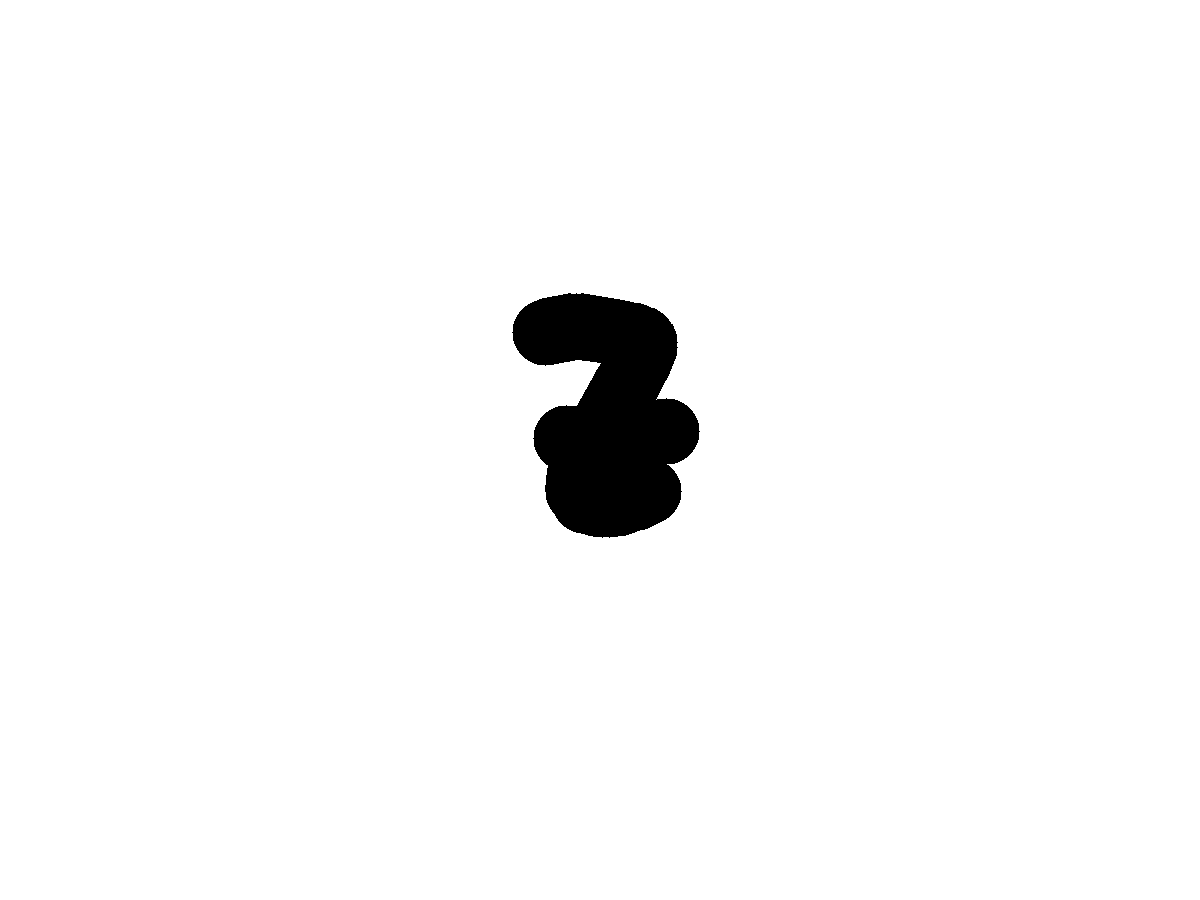
\includegraphics[width=\linewidth]{images/bad_char1}
  \caption{Picture of a 'z' which resembles a 7.}
\end{subfigure}
\begin{subfigure}{.23\textwidth}
  \centering
  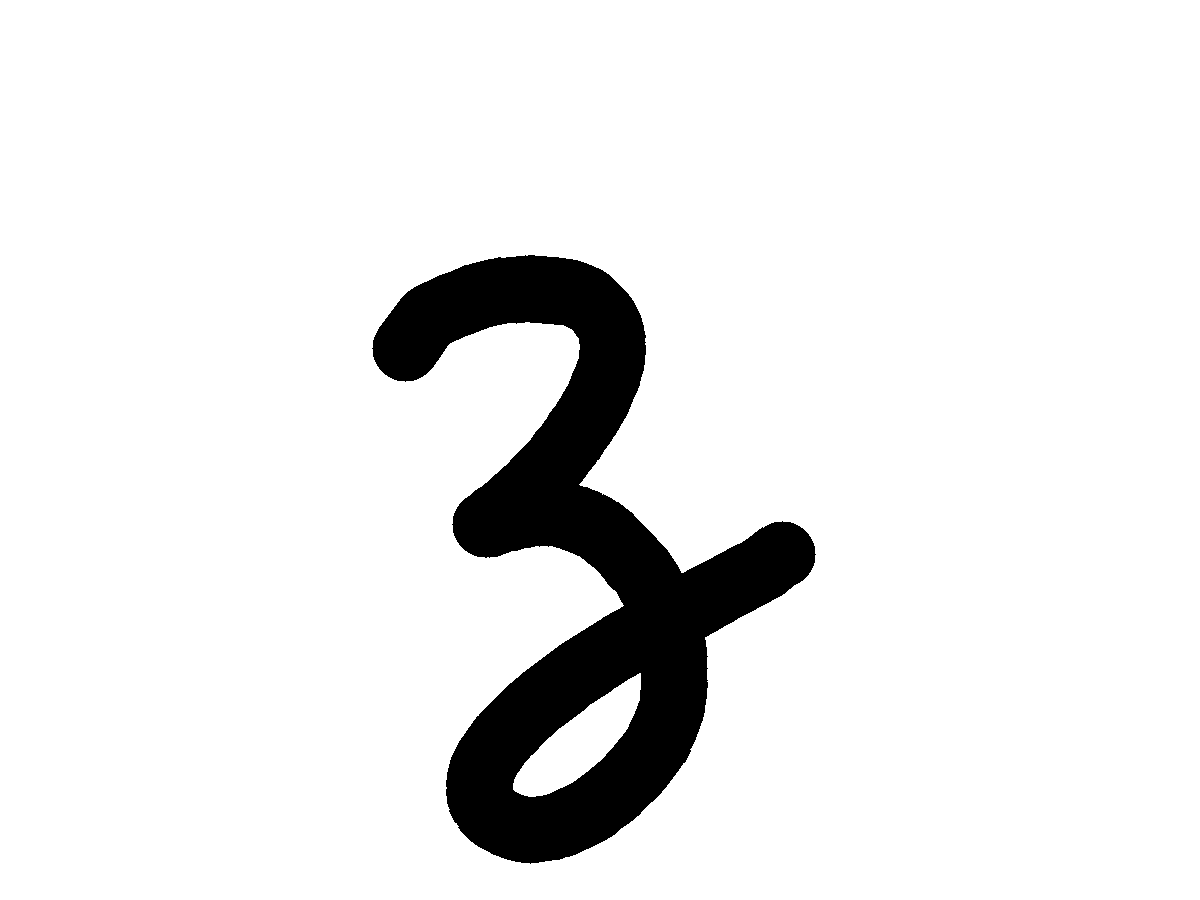
\includegraphics[width=\linewidth]{images/bad_char2}
  \caption{Picture of a 'z' which resembles a 3.}
\end{subfigure}
\caption{Examples of written 'z' characters, which are hard to recognise.}
\label{fig:char}
\end{figure}


\subsubsection{Preliminary steps}
\label{sec:preproc}
We make use of two types of preprocessing steps: normalization and augmentation of the data. Normalization of data adjusts the original data and data augmentation takes the data and uses augmentation techniques to create variations of the original data.

\paragraph{Normalizing data} 
\label{par:norm}
Theoretically feeding normalized data to the neural network returns the same output as before. 
In reality however, it's better to normalize data to avoid getting stuck in local optima and to increase training speed of the model \cite{NormGoal}.
We normalize the data by reducing the input dimensions from (1200,900,3) to (64,64,1). A simple threshold is added to improve the contrast in our image. 
This allows the foreground to be more distinguishable from the background and allows the neural network to train and recognise more easily. 

\paragraph{Augmenting data}
\label{par:aug}
Data augmentation serves two purposes. It makes the dataset more robust to different kinds of handwriting as we add variations of the original data to the input data. 
The second purpose is to increase the size of our dataset. As our dataset only contains 3410 images with handwritten characters, we need more data for the neural network to be able to function properly. 
Increasing the size of our dataset has great impact on the performance of the neural network as discussed in \ref{sec:expres}. Now we will describe the data augmentation techniques we used. For these techniques we based us on \cite{DataAug}. A more thorough explanation can be found there. 

\subparagraph{Adding noise to data}
We add a variant of each image which includes noise troughout the image with the purpose of reducing overfitting of the neural network \cite{DataNoise}. This noise is taken from the Gaussian distribution and summed with the original image.  
\subparagraph{Translations of data}
The dataset is also extended with variations in padding of characters in images. For this purpose we multiply every coordinate of the original image with the following transformation matrix: 
\begin{equation}
        \begin{bmatrix}
                1 & 0 & t_x \\
                0 & 1 & t_y
        \end{bmatrix}
\end{equation}
where $t_x$ is the horizontal shift and $t_y$ is the vertical shift. 
\subparagraph{Rotations of data}
Rotations of the image are added to the dataset to make the network more robust to handwritings with different orientations. We rotate by -30 and 30 degrees. This matrix is equal to:
\begin{equation}
       \begin{bmatrix}
               \alpha & \beta & (1-\alpha)*center.x - \beta*center.y \\
               -\beta & \alpha & \beta*center.x + (1-\alpha)*center.y
       \end{bmatrix}
\end{equation}
where $\alpha = cos(angle)$ and $\beta = sin(angle)$. Center is the coordinate in our image around which is rotated and the angle describes the amount of degrees to rotate in the clockwise direction. 
\subparagraph{Scaling of data}
With the purpose of making the network more robust to different sizes of handwriting, we add different scalings of the data. We both scale in width and in height. The following transformation matrix allows us to scale the input image: 
\begin{equation}
       \begin{bmatrix}
               s_x & 0 & 0  \\
               0 & s_y & 0
       \end{bmatrix}
\end{equation}
where $s_x$ is the horizontal scaling factor and $s_y$ is the vertical scaling factor. 
\subparagraph{Shearing of data}
In order to deal with different kinds of slants we add sheared versions of the image to the dataset. 
Shearing displaces each point in a fixed direction, by an amount proportional to its signed distance from a line that is parallel to that direction \cite{Shear}. We used the following shear mapping to achieve this: 
\begin{equation}
        \begin{bmatrix}
                1 & s & 0 \\
                0 & 1 & 0
        \end{bmatrix}
\end{equation}
\subparagraph{Erosion of data}
The erosion operation of images adds thinner versions of characters to the dataset. Erosion uses a kernel to convolute an image. 
The image is scanned using the kernel. The maximum pixel value of the overlapping part between the image and the kernel is computed. This pixel value of the anchor point of the kernel is replaced with the maximum pixel value. 
This causes bright regions to get thinner, and dark regions to get bigger in the image. A visualisation of this is shown in \ref{fig:erosion}. 
\begin{figure}
  \centering
  
\includegraphics[width=\linewidth]{images/erosion}
  \caption{Visualisation of eroding an inverted image with a handwritten 'j'. The right picture underwent erosion \cite{erosion}.}
\label{fig:erosion}
\end{figure}
All of the previously discussed preprocessing techniques are also applied to the eroded image. The final dataset contains translated, orientated, sheared, scaled and noisy versions of both the original image, and the eroded image. 
\subsubsection{Deep neural network}
\label{sec:dnn}

\paragraph{Introduction}
Humans have millions of connected neurons in the visual cortices which are capable of image processing.
We, humans, can recognise most characters without any thought because of this complex neural network inside our brain. 
For computers, character recognition is a more difficult task. We could try to write rule-based systems and define how every character should look like. This solution isn't flexible at all and is very hard to define.
We use a neural network, inspired by how the brain processes images. These deep neural networks contain several layers of connected perceptrons, where each connection is defined by weight and each perceptron is defined by a bias. 
The perceptrons take an input and calculate an output using an activation function. This allows perceptrons to make decisions. 
Normalized images can be fed to the neural network, which then propagate trough several layers and eventually produce as output the probabiliy that the input image has a certain class, one of the possible characters. 
Now follows a detailed overview of the actual deep neural network.

\paragraph{Convolutional layers}
 The input is a normalized image with one color channel. This is fed to a convolutational layer. Convolutional layers allow us extract features by scanning the image with filters. These features might be edges, corners, or any other type of shape in the image. The extracted features are called a feature map. 
 We can apply several of those filters using one convolutional layer to extract several types of features. 
 This works because images have spatial information, close pixels have shared information. By applying a filter, pixels in the same region will use shared biases and weights, which allows the filter to extract particular features. 
 Next we add a pooling layer, in particular a max-pooling layer. Pooling layers remove the positional information of the features in the image. This is useful because the exact location is less important than the location relative to the other features, and this allows us to reduce the amount of parameters required in the next layers. 
We use 3 convolutional layers combined with max pooling layers in order to extract low, medium, and high level features. 
\paragraph{Fully-connected layers}
Next we flatten the output of the last convolutional layer in order to extract a 1-dimensional array from the 3-dimensional feature maps. This 1-dimensional array can now be fed to a fully connected layer, which is a layer of connected perceptrons as previously discussed. 
There are 3 fully connected layers each connected with a dropout layer. The purpose of this layer is to remove activations at random. Dropout greatly reduces overfitting in the fully connected layers. We don't use this after the convolutional layers as they are very resistant to overfitting \cite{nnbook}. 
The last fully connected layer has 62 output neurons, which correspond to the 62 possible output classes. We use rectified linear units in order to compute the activation function.
\paragraph{Softmax layer}
 The last layer in the neural network is a softmax layer with a cross-entropy cost function. The softmax layer compute a probability distribution (a set of 62 numbers which sum up to 1) using the 62 output neurons from the previous layer. An element in the probability distribution estimates the chance of the input image to classify as a certain character. 
 The cross-entropy cost function uses the actual labels to calculate the error between the actual labels and the predicted labels (the previously discussed probabilities). The closer the cross-entropy function is to zero, the better it is at classifying handwritten characters.
 \paragraph{Weight adjustment}
Finally, in order to actually train the neural network, we need some kind of weight adjustment. This will effectively improve the decision making of perceptrons and thus, the classification of images. 
The Adam optimizer effectively fulfills this goal. In order to explain the Adam optimizer, a few other methods have to be known, a very brief explanation of these methods follow. 
First of all, stochastic gradient descent (SGD) is an iterative method which tries to find minima. This function takes a step size, which is known as the learning rate. SGD can be used to minimize the cross-entropy function iteratively by adjusting the weights. 
Momentum-based gradient descent makes the correction dependent based on an average of several previous corrections to move more quickly in the correct direction. 
AdaGrad allows the learning rate to adapt based on parameters. AdaDelta solves a problem of AdaGrad, concerning the learning rate to become so small that learning becomes impossible. 
Each of these methods effectively improve the previously mentionned method. 
The Adam optimizer is an optimization of AdaDelta, which uses a distinct learning rate and momentum for every parameter. This optimizer works best in our case and will be used. 

\subsection{Segmentation of text into words}
\subsection{Segmentation of words into characters}
\subsubsection{Correction of oversegmentation}
As our algorithm for segmentation of handwritten words splits the word into to many characters, we can use techniques to verify the correctness of these splitting points. 
\cite{evalsplitpoints} discusses 3 approaches to evaluate split point correctness: rule based approaches, cost function optimization based approaches and machine learning based approaches. 
In this paper we will only discuss the latter, machine learning based approaches, as we used this approach. 
In particular, our algorithm is based on \cite{evalsplitpointsnn}. The paper explains how to use neural networks to classify the correctness of splitting points. The discussed algorithm is as follows. Manual classification of splitting points creates training data with two classes, correct and incorrect splitting points. 
For every of these splitting points a pixel matrix is extracted surrounding the splitting point. This pixel matrix is normalised in size. 
Next, small windows of equal size are extracted from the pixel matrix and for each window the density is calculated. The is the number of black pixels divided by the total amount of pixels in the window. 
With every matrix a corresponding label is encoded for storage in the training file, this label is encoded as 0.9 if the splitting point is correct and 0.1 otherwise. Now these matrices and corresponding labels are used to train the neural network. 

We take a slightly different approach and consider a deep neural network to tackle this problem. This allows us to use convolutational layers in order to extract features, instead of manually creating features (features which show the density in this case). 
We use 1 convolutional layer and 3 fully connected layers in our neural network. This neural network takes the actual image of the splitting point as input (a pixel matrix of the pixels surrounding the splitting point) and returns a one-hot encoded vector indicating if the splitting is correct or incorrect. 
This allowed us to achieve better results than our implementation of the algorithm exactly as described by the paper achieved. Splitting points can now be filtered if the neural network decides a splitting point is incorrect. 


\subsection{Natural language processing}
To cope with some of the high error rates as shown in section \ref{sec:expres}, there needs to be some kind of correction. This correction should allow the system to produce possibble written text even when a step of the larger system fails. 
In order to do this we adapt natural language processing techniques as postprocessing steps. Natural language techniques can often be found in speech recognition, language generation and other systems. 
As a first step we match words against a dictionary to find out if they make sense, this is discussed in section \ref{sec:voc}. The second step checks if those given words make sense in the context, this is discussed in section \ref{sec:lm}.

\subsubsection{Vocabularium}
\label{sec:voc}
The neural network does not only produce which character is recognised, but rather a list of probabilities indicating the chance of an image to be a certain character. We can use all of this information in this postprocessing step instead of throwing that information away and naively returning the most likely character as the actual character. 
\begin{figure}
        \Tree [.{(Y, 0.9)} 
        [.{(Ye , 0.72)} {(Yes, 0.432)} {(Ye5 , 0.288)} ] 
        [.{(Yl , 0.18)} {(Yls, 0.108)} {(Yl5 , 0.072)} ]
            ] 
        \Tree [.{(T, 0.1)} 
        [.{(Te , 0.08)} {(Tes, 0.048)} {(Te5 , 0.032)} ] 
        [.{(Tl , 0.02)} {(Tls, 0.012)} {(Tl5 , 0.008)} ]
            ] 
\caption{A list of the trees for the word 'Yes' with branching factor 2. The characters have the following probabilities: $P(Y)=0.9, P(T)=0.1, P(e)=0.8, P(l)=0.2, P(s)=0.6, P(5)=0.4$. Other characters have probabilities which are neglible.}
\label{fig:wordtree} 
\end{figure} 
We make a tree, as shown in figure \ref{fig:wordtree}, where every node is a tuple with a word (sequence of characters) and a probability (likeliness of that word based on the probabilities of individual characters). The probability is calculated as the product of probability for each character: $P(c_1, c_2,...,c_k) = \prod\limits_{i}{c_i}$ with $1 \leq i \leq k$. In order to keep the complexity low we only consider the 3 most probable characters. This will be the branching factor of every tree. There's a tree for every possible starting character. 
Now we have a list of possible words and their probabilities (every leaf). The closest matches in the dictionary for each word are calculated using the function \textbf{get\_close\_matches} from the python library difflib. \textbf{get\_close\_matches} finds close matches in the English dictionary and their corresponding score. 
We multiply this score with our previously calculated probability. This leaves us with a list of correct English words and a score for every word. If we only want to convert the image of one word into text, we can just return the word with the highest score. 
This finalises the logic for recognising handwritten words. Next we will discuss a postprocessing technique useful we the word is part of a bigger context.
\subsubsection{Language model}
\label{sec:lm}
Besides checking the syntax of words, we can also look at the context. This is were language models are useful. We can check the previous words and calculate the likeliness of a word to be the next word in the context. N-gram models are used to calculate probabilities given n-1 previous words. The probability is computed as $P(w_i | w_{i-n},...,w_{i-1})$. 
We use the Markov assumption here: the probability of a word in the context can be approximated by the previous n-1 words. This probability is calculated as follows: 
\begin{equation}
        P(w_i | w_{i-n},...,w_{i-1}) = \frac{count(w_{i-n},...,w_{i-1},w_{i})}{count(w_{i-n},...,w_i)}
\end{equation}
where $w_i$ is the word of which we want to calculate the probability and $count(w_i,...w_{i+k})$ indicates the amount of occurences of $w_i,...,w_{i+k}$. That amount is the same as counting the amount of n-grams with that sequence of words. An n-gram is a sequence of n words from a given sequence of text, denoted as $w_i,...,w_{i+k}$.
We use the n-grams from the Google dataset for this purpose. Querying these datasets locally takes several minutes, and this happens for every word. Instead we use a Python library phrasefinder to make online queries to these corpora. This greatly increases speed but has the disadvantage of requiring internet connection. 
Now we can make queries such as "I like dogs / cats / sheep". Using the Google corpora probabilities are calculated with n-gram models for each of the 3 words. This gives us a probability for every word based on the context. 
Combining the results with the probabilities calculated in section \ref{sec:voc}, we can 
calculate a new score. The word with the highest score is accepted as written word. 
The concludes our full system of recognising handwritten texts. In the next section we will further discuss the results of these techniques and some experiments to check the performance and impact of optimizations. 
\section{Experimental results}
%TODO
\subsection{Character Recognition}
\label{sec:expres}
We tested a lot of different configurations for the deep neural network in order to find a good functioning neural network given the low amounts of data. A problem which arrised when trying to test many diffeent configurations was the long time it takes to train a neural network. In order to limit the time these experiments run we added some small constraints. Next it's important to note that a lot of non-determinism is part of these neural networks. When running the neural network twice with the same configuration, it could have completely different results. 
Another note is that some experiments might not use the finalized setup of our neural network. These experiments do use a same setup to compare different configurations. 
In order to have meaningful results which run in a reasonable amount of time we ran every experiment 4 times but limited the amount of epochs to 200. This setup is important to note, as some results might be quite different if we run more tests or use more iterations. When discussing these results we take the best result of the 4 training results. 
We use this result as we are only interested in the potential of the neural network, and not possible outliers which perform bad due to poor weight adjustments.  
\subsubsection{Experiments}
\paragraph{Preprocessing techniques}
Figure \ref{fig:preprocess} shows that preprocessing techniques have great influence on the performance of the neural network. We can see that the accuracy is much higher when using all of the preprocessing techniques.  
We achieve 72\% accuracy with all of the preprocessing techniques versus 35\% without any preprocessing techniques, which is a huge difference. 
We can also see the individual impact of preprocessing in the figure. Adding shearing (64\%) to handle different amounts of slant, adding noise (58\%) to cope to make the recognition more robust and adding scaling (59\%) to handle different handwriting sizes was the most effective to increase performance. Adding rotations (40\%) and translations (50\%) was less effective (but still effective). Adding these preprocessing techniques increased the amount of data greatly from 3410 examples to 37000 examples. This improves the performance but also increases the training time of our network significantly. One remarkable result is that the training time of preprocessing with all techniques enabled, takes shorter time than some other results. When we look at the average however, the training time is the highest for this case. 
\paragraph{Learning rate}
Figure \ref{fig:learningrate} shows the impact of learning rate on the training of our neural network. 
For this experiment we do have to note that we're using the Adam optimizer to train our neural network which computes individual learning rates for every parameter every training step. The learning rate which we pass is the initial learning rate. Choosing a high learning rate $10^-3$ allows the neural network to converge to a high accuracy (76 \%) very fast, but once reached the accuracy fails to grow any more.
This in contrast to higher learning rates which reach a good accuracy more slowly but find a more optimal solution. Learning rate $10^-4$ reaches an accuracy of 68\% after 200 iterations but is still growing. Learning rate $10^-5$ only reaches an accuracy of 5\% after 200 iterations but should find a better solution eventually than the other two configurations. 
\paragraph{Batch size}
In figure \ref{fig:batchsize} we can see the impact of choosing different batch sizes which are fed to the neural network. In order to increase to speed at which the neural network is trained, we feed batches of input images to the neural network instead of one image at a time. 
Weight adjustment only occurs after feeding a complete batch to the network. In the figure we can see bigger batch sizes increase the execution speed. However these differences are quites small. The configuration with batch size executes 200 iterations in one minute less than a configuration with batch size 128. These batch sizes also have an effect on our performance. When using small batch sizes backpropagation happens more frequently, which implies our weights will be more finetuned. The configuration with batch size 128 obtains an accuracy of 10\% higher than batch size 1024.
\paragraph{Weight decay}
In order to regulize the neural network we add weight decay to the network loss function in order to penalize big weights. The impact of different decays can be seen in \ref{fig:decay}. A high decay functions best (71\% accuracy) because we have a small amount of training examples. Without decay we only reach an accuracy of 65\%. 
\paragraph{Dropout}
% Maybe redo this experiment? It's not clear at all at this time whether dropout has an actual effect on the accuracy. I believe it helps find a better global solution, but often the accuracy will be lower as we're only using half of the weights. Further research is required. 
\begin{figure}
\centering
    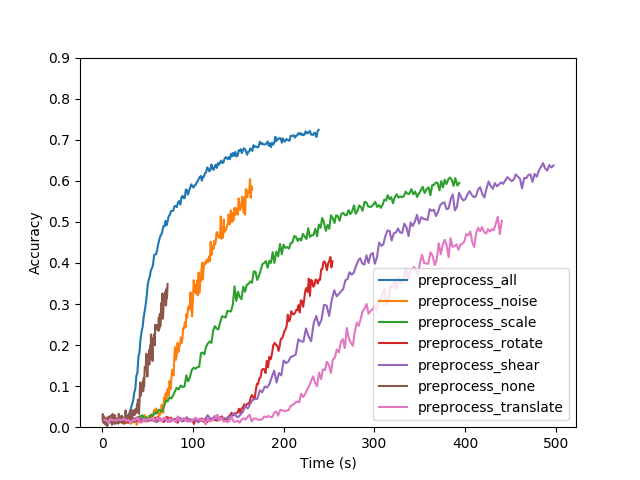
\includegraphics[width=\linewidth]{../Graphs/preprocess.png}
    \caption{Impact of various preprocessing techniques.}
    \label{fig:preprocess}
\end{figure}
\begin{figure}
    \centering
    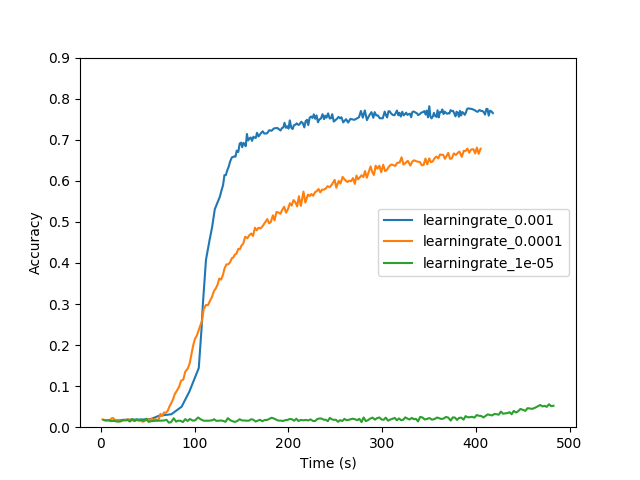
\includegraphics[width=\linewidth]{../Graphs/learningrate.png}
    \caption{Impact of different learning rates.}
    \label{fig:learningrate}
\end{figure}
\begin{figure}
    \centering
    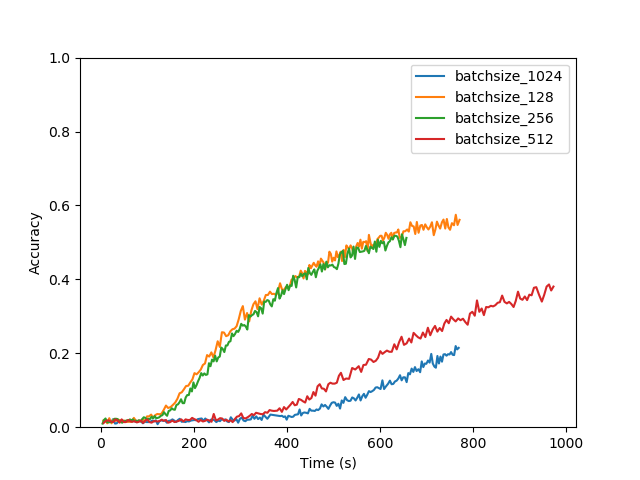
\includegraphics[width=\linewidth]{../Graphs/batchsize.png}
    \caption{Impact of different batch sizes.}
    \label{fig:batchsize}
\end{figure}
\begin{figure}
    \centering
    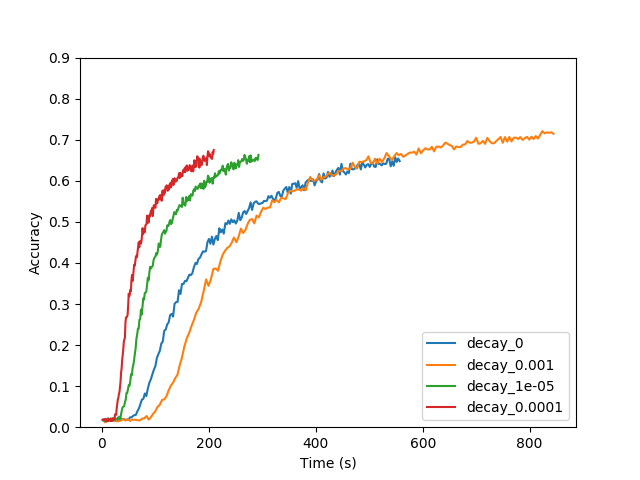
\includegraphics[width=\linewidth]{../Graphs/decay.png}
    \caption{Impact of weight decay regularisation.}
    \label{fig:decay}
\end{figure}
\subsubsection{Final results}
% Add graph with several runs of the final network. Discuss which parameters we took. 
% Maybe some more visualisation of mispredicted characters? Oh this isn't part of char recognition...
% TODO TODO
\section{Conclusion}

\section{Future research}

\bibliography{paper}
\bibliographystyle{icml2016}


\end{document} 
